\chapter{System architecture}
Well equipped with all the basic theoretical tools that we need, we can move on to implementing them for the game of Abalone. A first logical step would be to look at the existing software landscape to decide if we can utilize existing tools to speed up development.

\section{Software}
\subsection{Machine learning libray}
Machine learning projects share many components. Most commonly that is the declaration of the computational graph and the training of the graph. The libraries not only provide those components but also bring significant optimizations and specialized code for hardware acceleration. Therefore, it is imperative to decide on a suitable library to speed up development by several orders of magnitude.

\begin{figure}
    \centering
    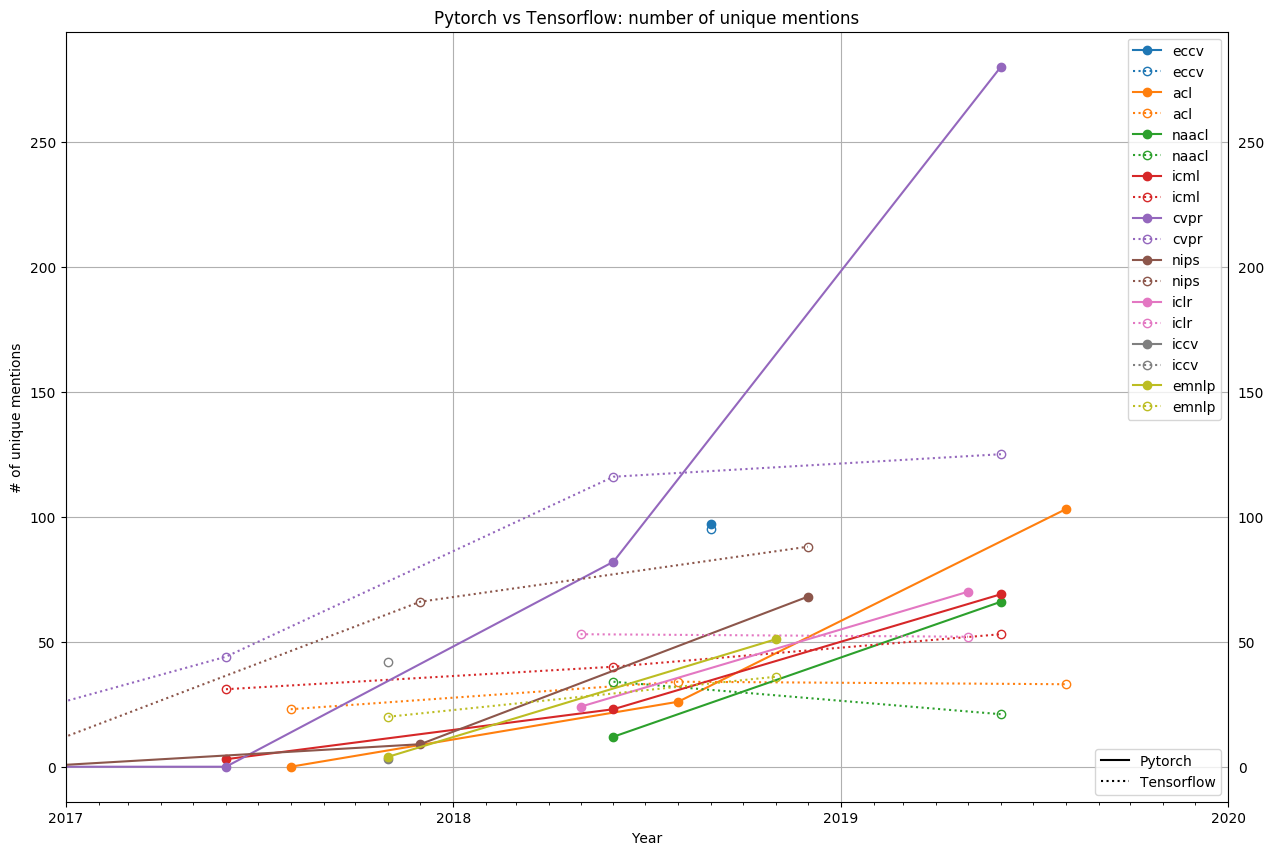
\includegraphics[height=7cm, keepaspectratio]{ml_framework_popularity.png}
    \caption{The mentions of pytorch and tensorflow in research papers in different publications \cite{noauthor_state_2019}}
    \label{ml_framework_popularity}
\end{figure}

A first indicator to go by is the popularity of the frameworks. Currently, the most relevant frameworks are Facebook's pytorch and Google's tensorflow. The Keras API has been introduced to tensorflow, therefore it is not considered further. In research pytorch seems to have quickly taken the dominance as depicted in figure \ref{ml_framework_popularity}. Aside from all differences between both libraries, the choice was guided by two practical reasons. Initially, tensorflow was selected due to the included support for TPUs as this project was granted free access to Google's Reseach Cloud \cite{noauthor_tpu_nodate}. At a later stage it became clear that Google was unwilling to increase the CPU quota for the account limiting the server to 8 cores which posed a significant problem for parallel execution.

As depicted in table \ref{pytorch_vs_tensorflow_performance} there is also a significant performance difference in the inference step of the MCTS. There are two ways in tensorflow to perform inference, either through the \texttt{predict} function or by calling the \texttt{\_\_call\_\_} method of the $model$ itself. As in the implementation the inference is not batched but done for individual board states, the usage of the latter option is faster \cite{noauthor_tfkerasmodel_nodate}. Nevertheless, pytorch is about five times faster. As discussed later, this is the reason to pivot to pytorch as framework.

\begin{table*}
    \begin{center}
        \begin{tabular}{ c|c|c|c|c }
            HW  & Framework & Neural net size & $\texttt{predict}(s)$ & $\texttt{\_\_call\_\_}(s)$ \\
            \hline
            \hline
            CPU & tf        & small           & ~0.027s               & ~0.011s                    \\
            GPU & tf        & small           & ~0.024s               & ~0.005s                    \\
            CPU & tf        & large           & ~0.027s               & ~0.015s                    \\
            GPU & tf        & large           & ~0.025s               & ~0.011s                    \\
        \end{tabular}
    \end{center}
    \caption{The average time ($n = 3,000$) taken to perform the feed-forward through the network for state $s$ with either ($\texttt{predict}(s)$) or ($\texttt{\_\_call\_\_}(s)$) in tensorflow}\label{tensorflow_predict_vs_call}
\end{table*}

\begin{table*}
    \begin{center}
        \begin{tabular}{ c|c|c|c|c }
            HW  & Framework & Neural net size & $\texttt{predict}(s)$ & $\texttt{search}(s)$ \\
            \hline
            \hline
            CPU & tf        & small           & ~0.01s                & ~0.016s              \\
            GPU & tf        & small           & ~0.005s               & ~0.011s              \\
            CPU & tf        & large           & ~0.014s               & ~0.02s               \\
            GPU & tf        & large           & ~0.011s               & ~0.017s              \\
            CPU & pytorch   & small           & ~0.005s               & ~0.011s              \\
            GPU & pytorch   & small           & ~0.001s               & ~0.007s              \\
            CPU & pytorch   & large           & ~0.005s               & ~0.011s              \\
            GPU & pytorch   & large           & ~0.002s               & ~0.008s              \\
        \end{tabular}
    \end{center}
    \caption{The average time ($n = 3,000$) taken to perform the feed-forward through the network for state $s$ ($\texttt{predict}(s)$) and one iteration of MCTS ($\texttt{search}(s)$)}\label{pytorch_vs_tensorflow_performance}
\end{table*}

\subsection{Training framework}
As there are existing frameworks that have implemented the system described in the AlphaZero paper in a more general and adaptable fashion, it has to be considered building on their foundation:
\begin{itemize}
    \item AlphaZero General is a framework developed as a university project at Standford originnally for the game of Hex and Othello. \cite{thakoor_learning_nodate,thakoor_suragnairalpha-zero-general_nodate}.
    \item Deep MCTS is a framework developed in the context of a Master's thesis \cite{bruasdal_deep_2020,henribru_deep_2021}.
\end{itemize}

To compare both options a catalogue of criteria is considered. Parallel training and parallel search measure whether the software implements the parallel training pipeline and MCTS-APV proposed by the AlphaZero paper. Moreover, it is checked whether the libraries are agnostic to the game and ML library that is being used. Lastly, it is relevant to investigate whether the performance could be verified by other users.

\begin{table*}
    \begin{center}
        \begin{tabular}{ c|c|c }
            Criterion             & AlphaZero General & Deep MCTS \\
            \hline
            \hline
            Parallel training     & 0                 & 1         \\
            Parallel search       & 0                 & 0         \\
            ML library agnostic   & 1                 & 0         \\
            Game library agnostic & 1                 & 1         \\
            Verified performance  & 1                 & 0         \\
            Simplicity            & 1                 & 0         \\
            \hline
            \hline
            Sum                   & 4                 & 2         \\
        \end{tabular}
    \end{center}
    \caption{A comparison of existing AlphaZero frameworks}\label{training_framework_comparison}
\end{table*}

As shown by table \ref{training_framework_comparison}, the winner by those criteria is AlphaZero General. Core advantages of the library are its simplicity and popularity. Deep MCTS makes use of a lot of abstractions and generics which makes the code more professional and reusable but provided also significant difficulties in understanding. The application of AlphaZero General to multiple other games like Gobang, Santorini, Connect4 etc. have shown its performance. The major drawback is the lack of a parallelized training pipeline.

\subsection{Game library}
There are two relevant implementations of game libraries for Abalone. As the interfacing language for pytorch is Python it makes sense to restrict the libraries to Python.

\begin{itemize}
    \item Abalone-BoAI is a game library that is specifically designed for interfacing with computational agents. It is very simple and has been used for the precursor project of this thesis \cite{scriptim_scriptimabalone-boai_2021}.
    \item Gym-abalone is tightly integrated with OpenAI's gym allowing agents to potentially play other games as well. The API is more designed for the reinforcement learning setting \cite{towzeur_towzeurgym-abalone_2021}.
\end{itemize}

Two arguments lead to the decision of choosing Abalone-BOAI:
\begin{enumerate}
    \item It was already optimized in the previous project as the generation of legal moves is computationally expensive.
    \item The API of the engine needs to be adapted to fit the interface of the training framework, wherefore intricate knowledge of the engine is of advantage.
\end{enumerate}

As mentioned in the section \ref{existing_game_playing_agents}, Verloop's reimplementation \cite{verloop_abaloneai_nodate} offers the simplest solution for interfacing with (one of) the strongest Abalone algorithms. In a small tournament personal implementations of minimax in Python \cite{claussen_abalone_2021} were inferior. This creates the necessity of interfacing between Java and Python. As the Java implementation is tightly coupled with with the internal game-engine it was decided to implement a proxy player for each game-engine. The proxy players communicate through a named pipe as depicted in figure \ref{python_java_ipc}. The downside of this solution is the need of synchronizing two separate game states.

\begin{figure}
    \centering
    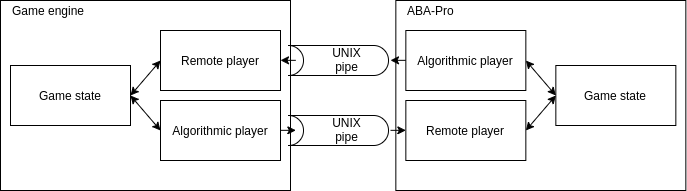
\includegraphics[height=4cm, keepaspectratio]{game_engine_communication.png}
    \caption{The inter process communication between the python game engine and the Java implementation of ABA-PRO}
    \label{python_java_ipc}
\end{figure}

As both implementation have a differing move notation an intermediary string-based format was introduced to serialize the moves more easily. The regex for the format is the following:

\begin{BVerbatim}
    [A-I][1-9]){1}([A-I][1-9]){0,1}((NE)|(E)|(SE)|(SE)|(SW)|(W)|(NW)){1}
\end{BVerbatim}

This means that inline moves have the structure of "{MarbleCoordinate}{Direction}" and broadside moves the structure of "{MarbleCoordinate}{MarbleCoordinate}{Direction}". Additionally, the marble coordinates are ordered for broadside moves. The marble coordinates outlined in figure . The directions are always seen from the white players starting positon, north pointing straight in the direction of the black player (default position).

\section{Neural network}
The neural network architecture of the

\begin{figure}
    \centering
    \begin{BVerbatim}
        0 1 2 3 4 5 6 7 8
        0          o o o o o
        1        o o o o o o
        2      · · o o o · ·
        3    · · · · · · · ·
        4  · · · · · · · · ·
        5  · · · · · · · ·
        6  · · @ @ @ · ·
        7  @ @ @ @ @ @
        8  @ @ @ @ @
    \end{BVerbatim}
    \caption{The matrix representation of the hexagonal field}
\end{figure}

\begin{figure}
    \centering
    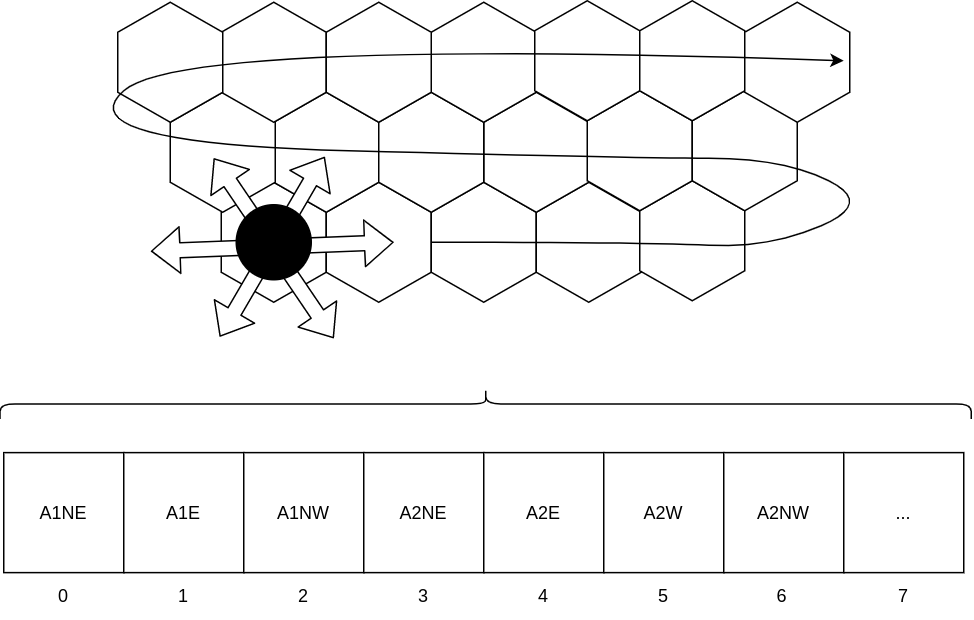
\includegraphics[width=13cm, keepaspectratio]{possible_move_generation_inline.png}
    \caption{}
    \label{possible_move_generation_inline}
\end{figure}

\begin{figure}
    \centering
    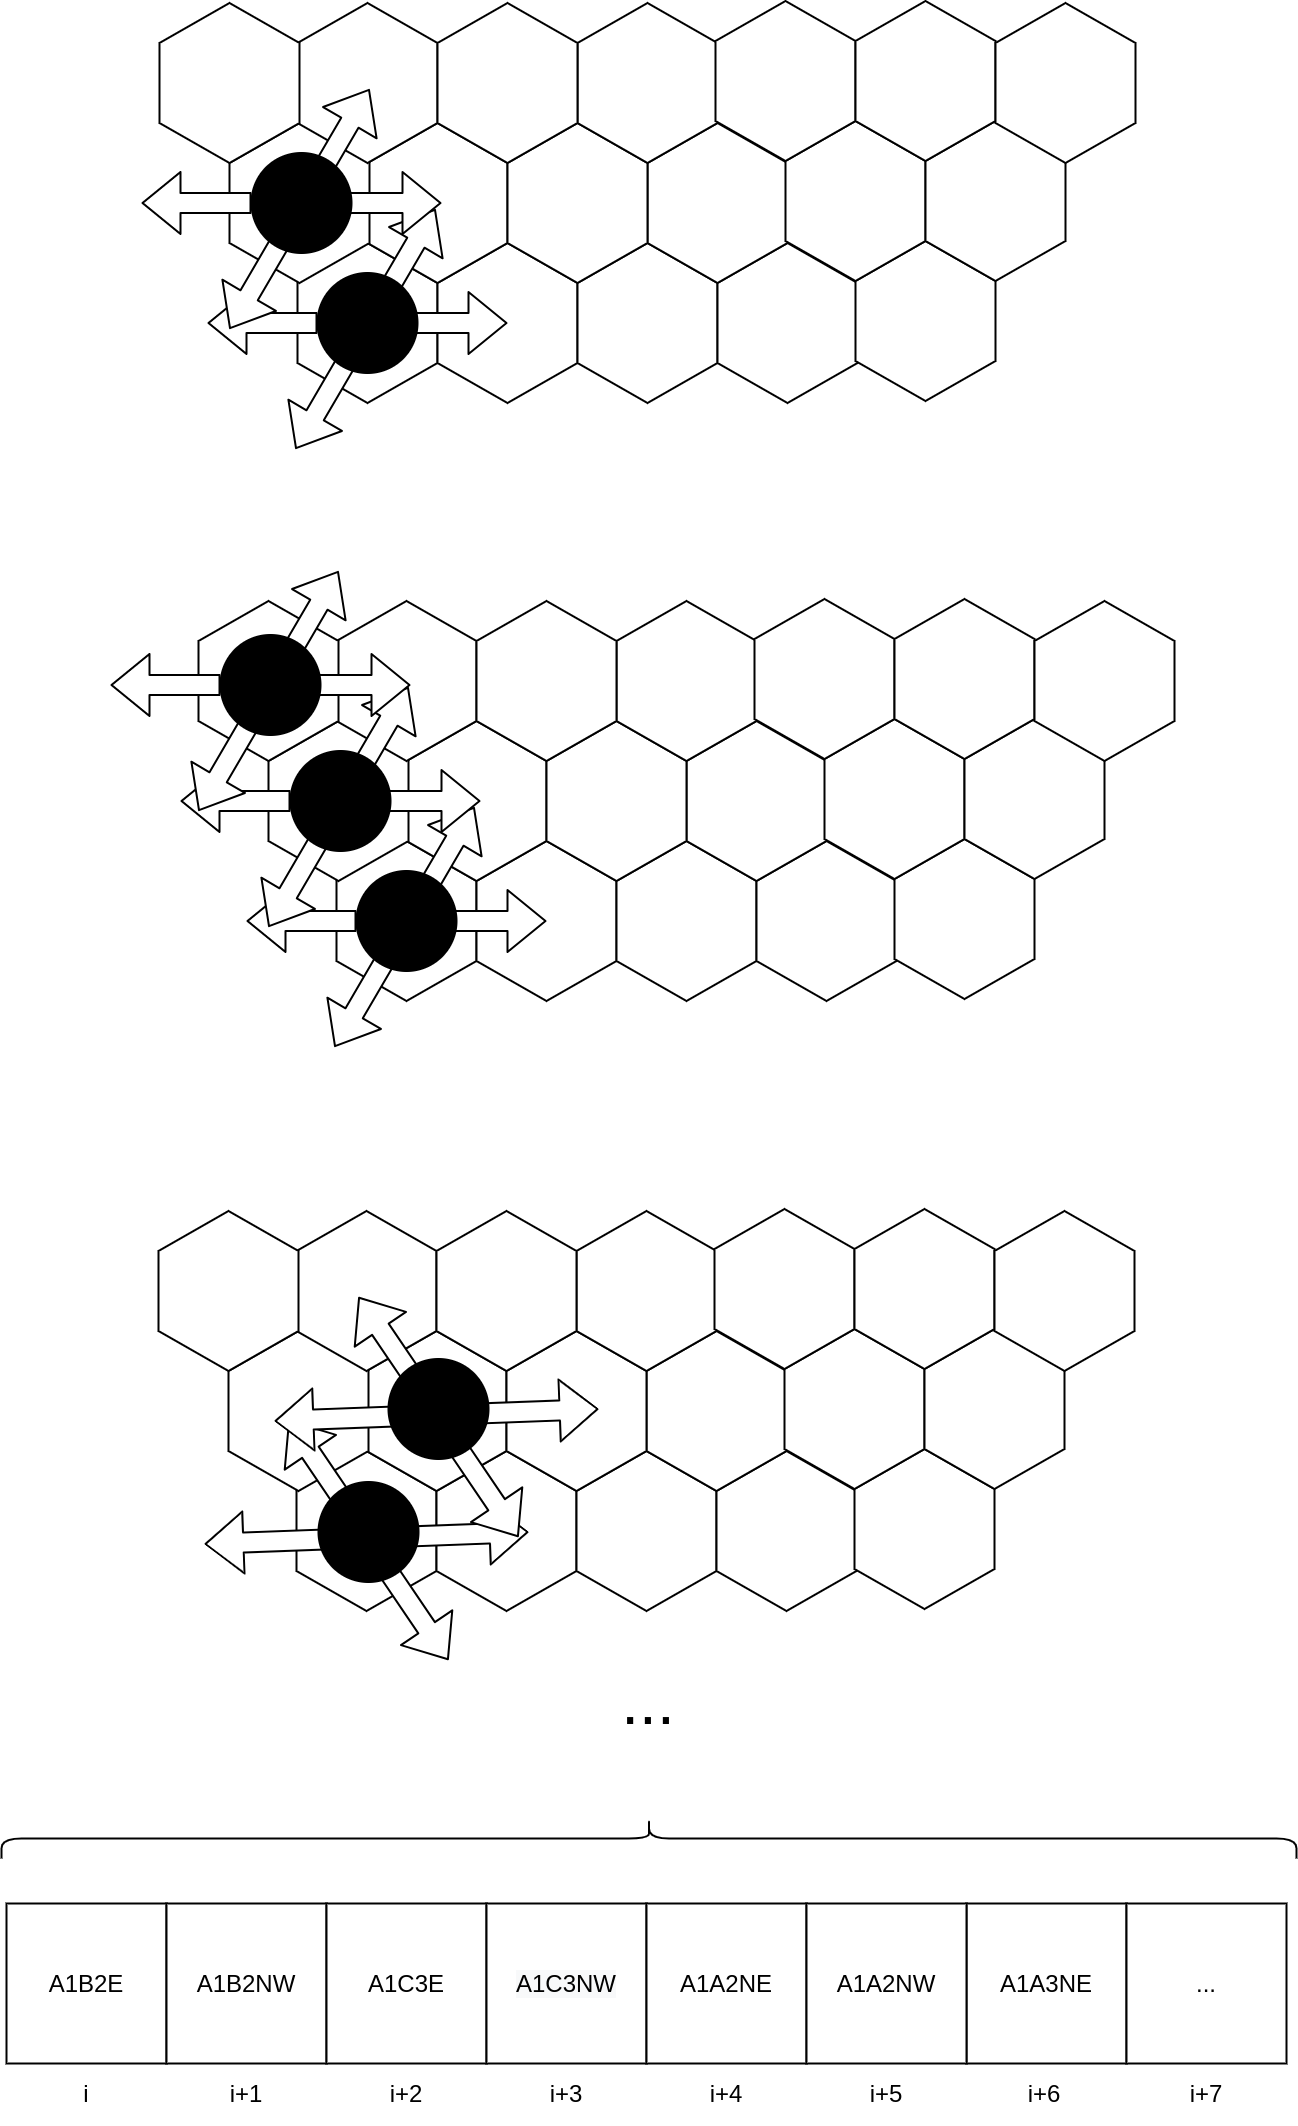
\includegraphics[width=13cm, keepaspectratio]{possible_move_generation_broadside.png}
    \caption{}
    \label{possible_move_generation_broadside}
\end{figure}

\section{Training pipeline}
\begin{figure}
    \centering
    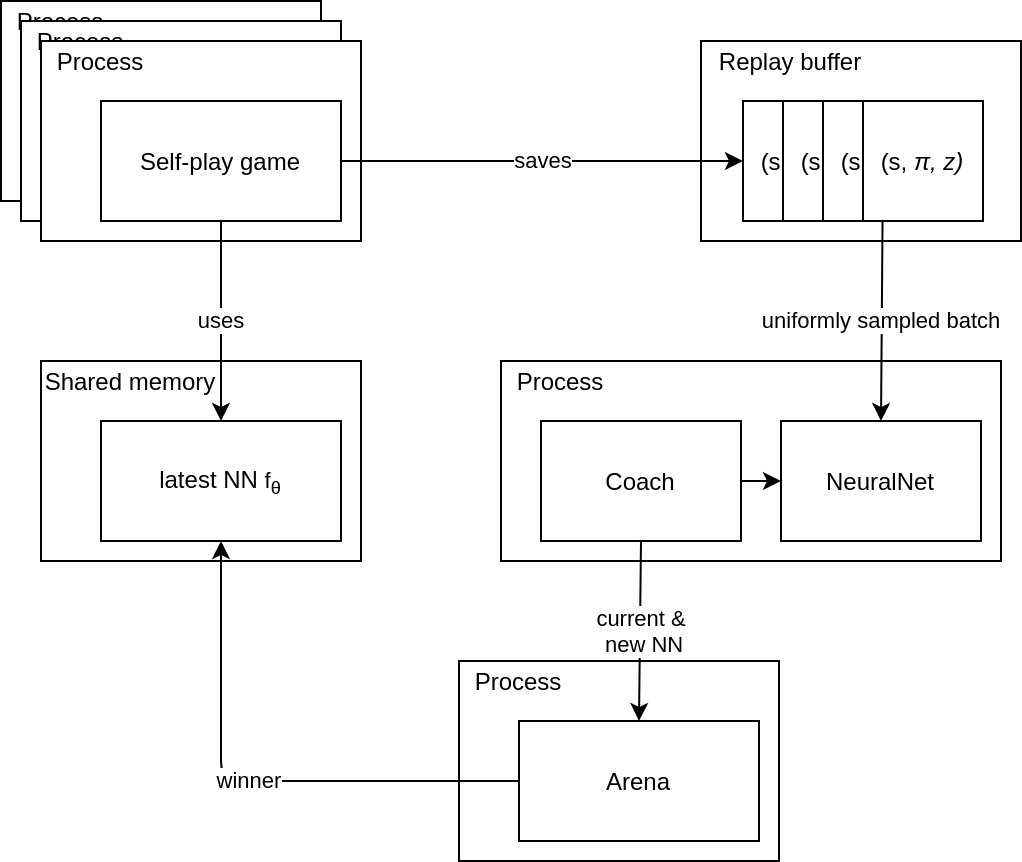
\includegraphics[height=10cm, keepaspectratio]{parallel-training.png}
    \caption{The different processes during the parallel training}
    \label{parallel_training_pipeline}
\end{figure}

\begin{figure}[!h]
    \centering
    \subfloat[The main loop of the training algorithm]{
        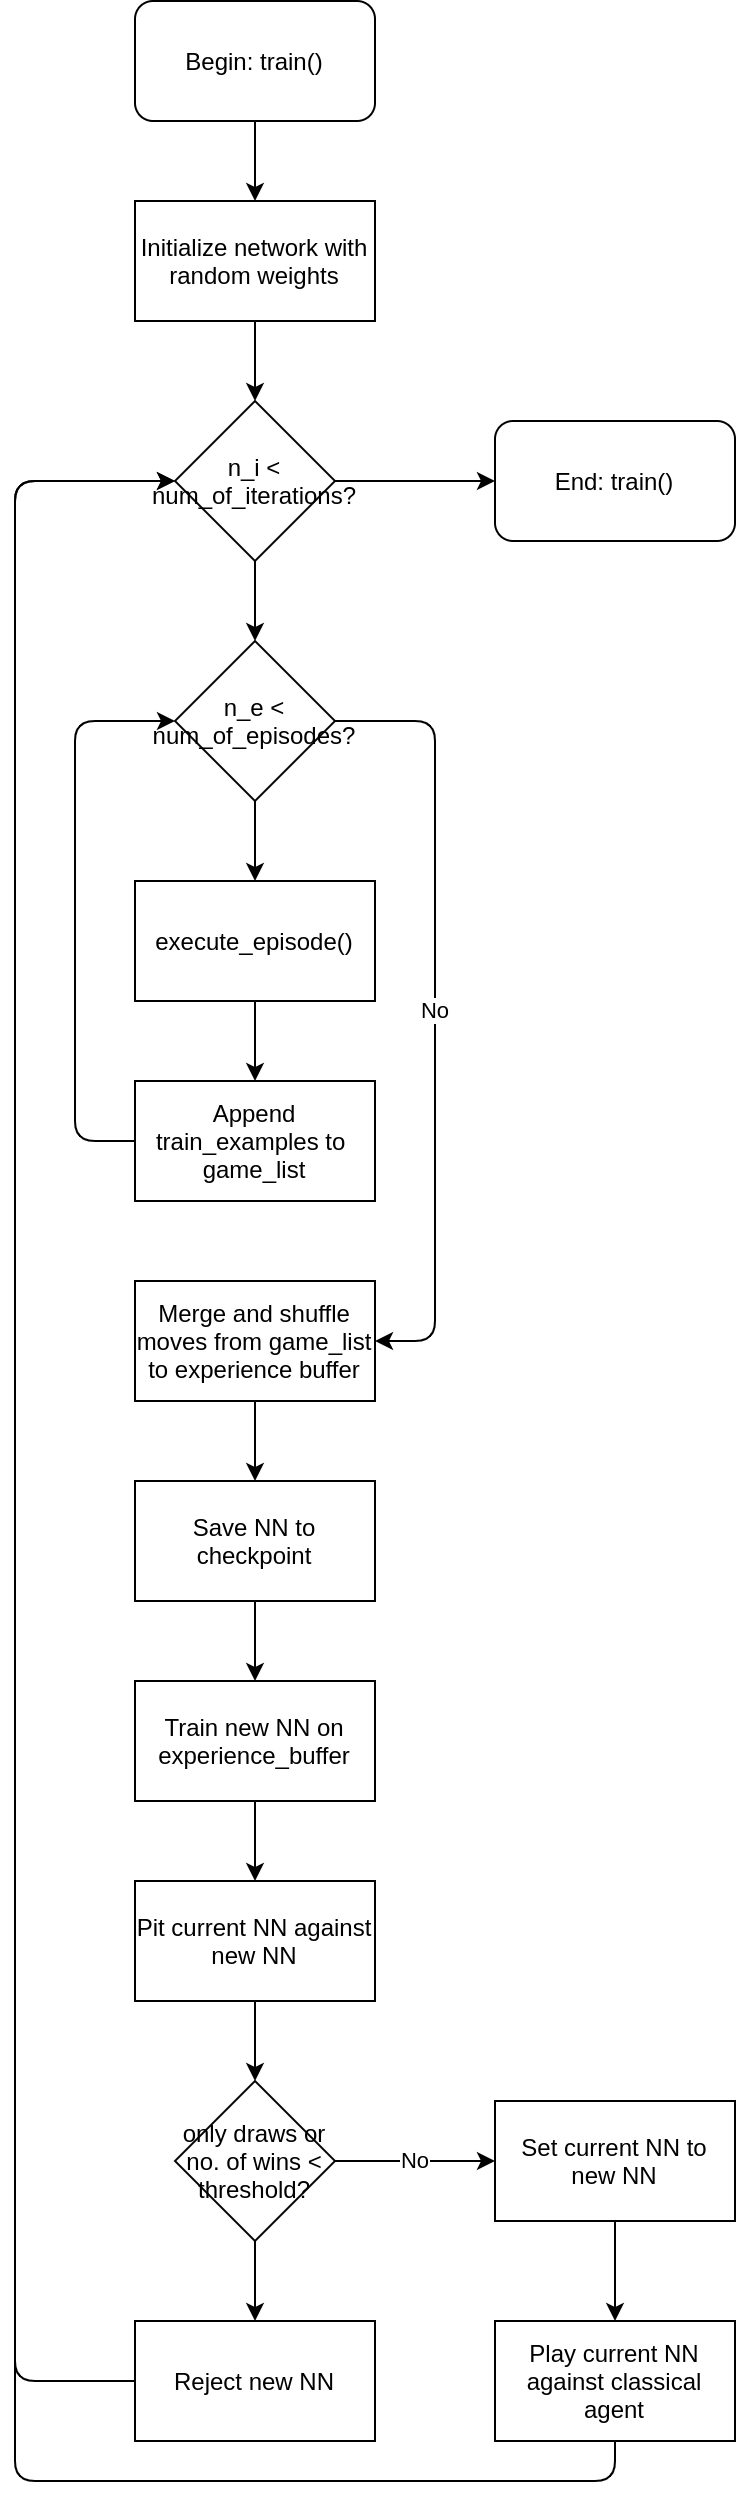
\includegraphics[width=6cm, keepaspectratio]{training_main_loop.png}
    }
    % \hfill
    \subfloat[The episode loop]{
        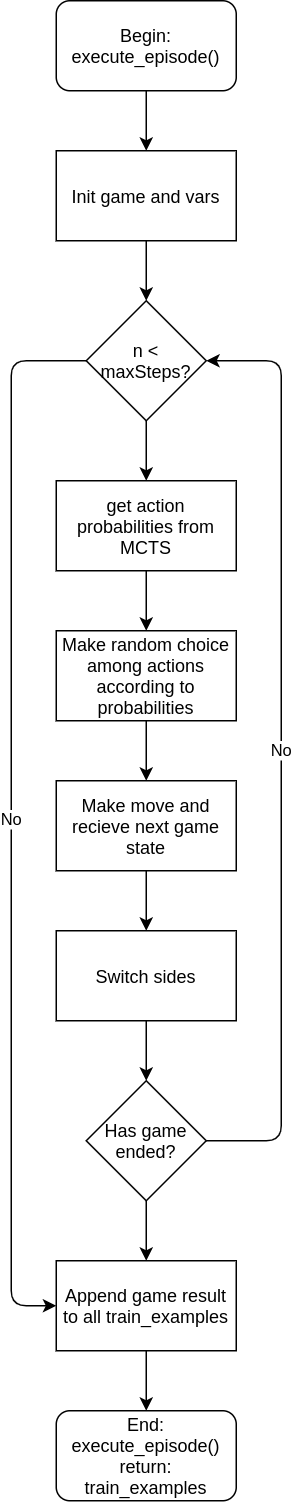
\includegraphics[width=4cm, keepaspectratio]{training_episode.png}
    }
    \caption{The self-play training pipeline}
    \label{training_algorithm}
\end{figure}
